\chapter{Where4 System Overview and Data Collection}% Main chapter title
\thispagestyle{nohead}
\label{Experimental} % For referencing the chapter elsewhere, use \ref{experimental} 

Empirical studies require many choices to be made from the outset. In the case of \where, the following questions were identified:

\begin{enumerate}
	\item Which solving back-ends of \why should be supported by \where?
	\item What program data should the machine learning algorithm use for training and testing?
	\item What are the predictor variables to be extracted from these programs?
	\item What is to be predicted by the machine learning algorithm?
	\item How is the accuracy of response variables to be ensured?
	\item Which machine learning algorithm should be used by \where?
	\item How is \where's interaction with \why implemented?   
\end{enumerate}   

In this chapter we detail the tools and data chosen to be measured and the methods used for this measurement; i.e. questions 1-5 are answered. Question 6 is answered in Chapter \ref{Prediction}. The choices made in regard to Question 7 are discussed in Chapter \ref{Implementation}. 

A diagram illustrating this part of the experimental process is given in Fig. \ref{fig:Chapter3}. In Sec. \ref{sub:why3programs} the import formats supported by \why are discussed and the repository of verification programs used for training and testing purposes are introduced. The selection of SMT-solving tools considered by this study is discussed in Sec \ref{sub:smtselection}.  

The next subsection, Sec. , details the process taken to extract a number of structural code-based metrics from the proof obligations sent to the SMT solvers by \why.  

The accurate measurement of SMT solver execution time is important for training data to reflect actual tool behaviour. The steps taken to ensure the response variables were statistically representative are given in Sec. . 

\begin{figure}
\centering
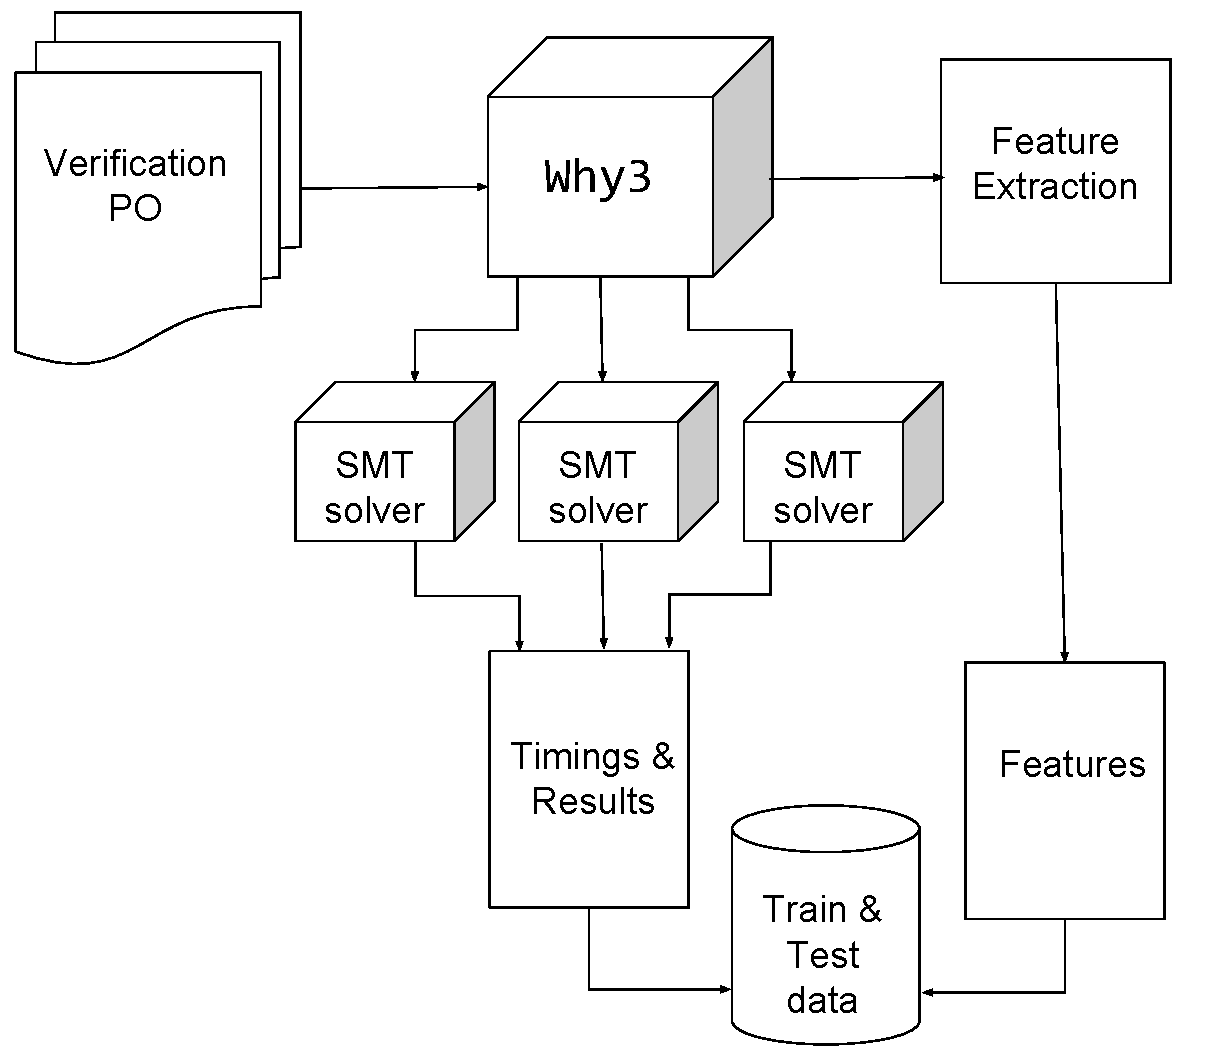
\includegraphics[width=0.9\linewidth]{Figures/Chapter3}
\caption{Diagram illustrating the process to collect predictor and response variables for the \where model}
\label{fig:Chapter3}
\end{figure}

\section{Selection of tools and programs}
\label{sec:selection}

\subsection{Selection of \why programs}
\label{sub:why3programs}

Due to the diverse range of input languages used by software verification systems, a standardised benchmark repository of verification programs does not yet exist \cite{Dagstuhl}.
For our study we chose the 128 example programs included in the \textsf{Why3} distribution (version 0.87.1) as our corpus for training and testing purposes. The programs in this repository are written in WhyML, a dialect of ML with added specification syntax and verified libraries. Many of the programs are solutions to problems posed at software verification competitions such as VerifyThis \cite{verifythis}, VSTTE \cite{Klebanov2011} and COST \cite{bormer:hal-00789525}. Other programs are implementations of benchmarks proposed by the VACID-0 \cite{Leino10vacid-0:verification} initiative.   It is our assumption that these programs are a representative software verification workload. Alternatives to this dataset are discussed in Section \ref{sec:related}. 

\subsection{Selection of \textsc{SMT} solvers}
\label{sub:smtselection}

We used six current, general-purpose SMT solvers supported by \textsf{Why3}: Alt-Ergo \cite{AltErgo}, CVC3 \cite{CVC3}, CVC4 \cite{CVC4}, veriT\footnote{The most recent version - 201506 - is not officially supported by \why but is the only version available} \cite{veriT}, Yices\footnote{We did not use Yices2 as its lack of support for quantifiers makes it unsuitable for software verification} \cite{Yices}, and Z3 \cite{Z3}. We expanded the range of solvers to eight by also recording the results for two of the most recent major versions of two popular solvers - Alt-Ergo and Z3.


\begin{figure}
	\centering
	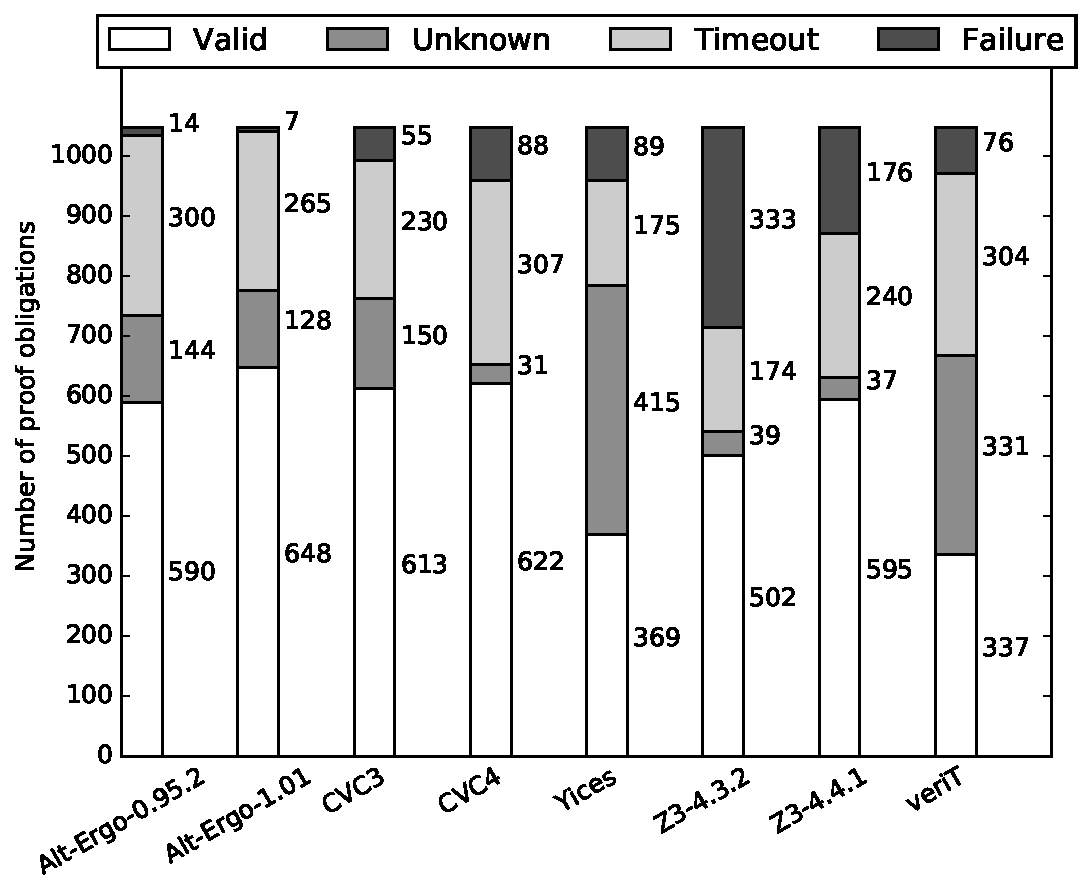
\includegraphics[width=0.8\linewidth]{barcharts}
	\caption{The relative amount of Valid / Unknown / Timeout / Failure answers from the eight SMT solvers (with a timeout of 60 seconds). Note that no tool returned an answer of Invalid for any of the 1048 proof obligations.}
	\label{fig:barcharts}
\end{figure}

When a solver is sent a goal by \textsf{Why3}, it returns an answer $A$ where $A$ is one of $\lbrace Valid,Invalid,Unknown,Timeout,Failure \rbrace$. As can be seen from Table \ref{table:avgtimes} and Fig. \ref{fig:barcharts}, not all goals can be proved Valid or Invalid. Such goals usually require the use of an interactive theorem prover to discharge goals that have been inductively defined. Sometimes a splitting transformation needs to be applied to simplify the goals before they are sent to the solver. Our tool does not perform any transformations to goals other than those defined by the solver's \textsf{Why3} driver file. In other cases, more time or memory resources need to be allocated in order to return a conclusive result. We address the issue of resource allocation in Section \ref{sec:independant}.     


\subsection{Problem Quantification: predictor and response variables}

Two sets of data need to be gathered in supervised machine learning \cite{Mitchell}: the independent/predictor variables which are used as input for both training and testing phases, and the dependent/response variables which correspond to ground truths during training. Of the 128 programs in our dataset, 25\% were held back for system evaluation (Section \ref{sec:eval}). The remaining 75\% (corresponding to 96 WhyML programs, 768 goals) were used for training and 4-Fold cross-validation.

\section{Independent/Predictor variables}
\label{sec:independant}

\subsection{Extracting static metrics from \why proof obligation formul\ae}
\label{sub:extracting}
%Using the \why notion of "goal shape"
Fig. \ref{fig:types} lists the predictor variables that were used in our study.  All of these are (integer-valued) metrics that can be calculated by analysing the \textsf{Why3} goal statement, and are similar to the \textit{Syntax} metadata category for proof obligations written in the TPTP format \cite{TPTP}. To construct a feature vector from each task sent to the solvers, we traverse the abstract syntax tree (AST) for each goal and lemma, counting the number of each syntactic feature we find on the way. We ignore the other contextual features such as axiom and predicate definitions as these are not sent to the solver. 

Our feature extraction algorithm has similarities in this respect to the method used by \textsf{Why3} for computing goal ``shapes'' \cite{why:preserving}. These shape strings are used internally by \textsf{Why3} as an identifying fingerprint. Across proof sessions, their use can limit the amount of goals in a file which need to be re-proved.   

\begin{figure}
	\centering
	\begin{tikzpicture}[
	level 1/.style={sibling distance=30mm},
	edge from parent/.style={->,draw},
	>=latex]
	
	\node[root]{Size}
	child {node[level 2] (c0) {ops}
		child {node[level 2, yshift=10pt] (c1) {divisor}}
		child {node[level 2, yshift=10pt] (c2) {conds}}
	}
	child {node[level 2, yshift=-32pt, xshift=55pt] (c3) {leaves}}
	child {node[level 2, yshift=-32pt, xshift=55pt] (c4) {quants}}
	;
	
	\begin{scope}[every node/.style={level 3}]
	\node [below of = c1, xshift=5pt, yshift=10pt] (c11) {and};
	\node [below of = c11, yshift=10pt] (c12) {or};
	\node [below of = c12, yshift=10pt] (c13) {not};
	\node [below of = c13, yshift=10pt] (c14) {let};
	\node [below of = c14, yshift=10pt] (c15) {as};
	\node [below of = c15, yshift=10pt] (c16) {eps};
	\node [below of = c16, yshift=10pt] (c17) {func};
	
	
	\node [below of = c2, xshift=5pt, yshift=10pt] (c21) {if};
	\node [below of = c21, yshift=10pt] (c22) {iff};
	\node [below of = c22, yshift=10pt] (c23) {imp};
	\node [below of = c23, yshift=10pt] (c24) {case};
	
	
	\node [below of = c3, xshift=5pt, yshift=10pt] (c31) {var};
	\node [below of = c31, yshift=10pt] (c32) {true};
	\node [below of = c32, yshift=10pt] (c33) {false};
	\node [below of = c33, yshift=10pt] (c34) {while};
	\node [below of = c34, yshift=10pt] (c35) {zero-ar};
	\node [below of = c35, yshift=10pt] (c36) {int};
	\node [below of = c36, yshift=10pt] (c37) {float};
	
	
	\node [below of = c4, xshift=5pt, yshift=10pt] (c41) {forall};
	\node [below of = c41, yshift=10pt] (c42) {exists};
	
	\node [below of = c42](c43) {depth};
	\node [below of = c43](c44) {avg-arity};
	
	\end{scope}
	% lines from each level 1 node to every one of its "children"
	\foreach \value in {1,...,7}
	\draw[->] (c1.195) |- (c1\value.west);
	
	\foreach \value in {1,...,4}
	\draw[->] (c2.195) |- (c2\value.west);
	
	\foreach \value in {1,...,7}
	\draw[->] (c3.195) |- (c3\value.west);
	
	\foreach \value in {1,...,2}
	\draw[->] (c4.195) |- (c4\value.west);
	
	\end{tikzpicture}
	\caption{Tree illustrating the Why syntactic features counted individually (\textit{pink nodes}) while traversing the AST. The rectangles represent individual measures, 
		and the rounded blue nodes represent metrics that are the sum of their children in the tree.}
	\label{fig:types}
\end{figure}



%\begin{table}
%\caption{Static metrics derived from \textit{Why} goal statements}

%\begin{tabularx}{\textwidth}{@{}lll@{}} 
%\toprule
%\textbf{Category}&\textbf{Metric}&\textbf{Explanation} \\ 
%\midrule
%\textsc{operators}
%&\texttt{and}&\\ &\texttt{or}&\\ &\texttt{not}&\\ &\texttt{let}&\\ &\texttt{as} &\\ &\texttt{eps}& epsilon operator\\ &\texttt{func}&user/library function call with variable arity \\ 
%\midrule
%\textsc{conditions}
%&\texttt{if}&\\ &\texttt{iff}&\\ &\texttt{imp}&implication\\ &\texttt{case}&variable arity \\
%\midrule
%\textsc{leaves}
%&\texttt{var}& Bound/unbound variable \\&\texttt{true}&\\&\texttt{false}&\\&\texttt{wild}&\\&\texttt{int}&integer constant\\&\texttt{float}&floating point constant\\ 
%\midrule
%\textsc{quantifiers}
%&\texttt{forall}& \\&\texttt{exists}& \\ 
%\midrule
%\textsc{cumulative}
%&\texttt{divisor} & sum of types in \textsc{operators}\\
%&\texttt{zero\_ar} & sum of \texttt{func} with an arity of 0\\
%&\texttt{conds} & sum of types in \textsc{conditions}\\
%&\texttt{leaves} & sum of types in \textsc{leaves} + \texttt{zero\_ar} \\
%&\texttt{quants} & sum of types in \textsc{quantifiers}\\
%&\texttt{size}&\texttt{divisor} + \texttt{leaves} + \texttt{conds} + \texttt{quants} - \texttt{zero\_ar} \\ 
%&\texttt{ops}&(\texttt{size} - \texttt{quants} + \texttt{leaves}) \\
%\midrule
%\textsc{other} & \texttt{depth} & depth of the parse tree \\
%&\texttt{avg\_arity}&(total arity of types in \textsc{operators} divided by \texttt{divisor} \\

%\bottomrule

%\end{tabularx}
%\label{table:types}
%\end{table}

\section{Dependent/Response variables}
%Measurement of dynamic properties
\label{sec:dependant}

Our evaluation of the performance of a solver depends on two factors: the time taken to calculate that result, and whether or not the solver had actually proven the goal.

\subsection{Execution time}
%mention the rationale behind choosing 10 seconds as a reasonable time limit
\subsubsection{Accounting for randomness with confidence intervals}

In order to accurately measure the time each solver takes to return an answer, we used a measurement framework specifically designed for use in competitive environments. The BenchExec \cite{benchexec} framework was developed by the organisers of the SVCOMP \cite{SVCOMP} software verification competition to reliably measure CPU time, wall-clock time and memory usage of software verification tools. We recorded the time spent on CPU by each SMT solver for each proof obligation. To account for random errors in measurement introduced at each execution, we used the methodology described by Lilja \cite{LiljaJ} to obtain an approximation of the true mean time. A 90\% confidence interval was used with an allowed error of $\pm$3.5\%.   



%By inspecting our data, we saw that most \textit{Valid} and \textit{Invalid} answers returned very quickly, with \textit{Unknown} answers taking slightly longer, and \textit{Failure/Timeout} responses taking longest. We took the relative utility of responses to be $Valid >$ $Invalid>Unknown>Timeout>Failure$ which can be read as ``it is better for a solver to return a \textit{Valid} response than \textit{Timeout}'', etc. A simple function allocates a cost to each solver $S$'s response to each goal $G$:
%\[\small
%cost(S,G) = 
%\begin{cases}
%time_{S,G}, \text{ if answer}_{S,G} \in \lbrace Valid, Invalid \rbrace \\
%time_{S,G} + \text{timeout}, \text{ if answer}_{S,G} = Unknown \\
%dist((time_{S,G},\text{timeout}), (0,0)), \text{if answer}_{S,G} \in \lbrace Timeout, Failure \rbrace
%\end{cases}
%\]
%
%Thus, to penalise the solvers that return an \textit{Unknown} result, the timeout limit is added to the time taken, while solvers returning \textit{Timeout} or \textit{Failure} are further penalised by taking the Euclidean distance from $(0,0)$ to the point defined by the (time taken, timeout limit). This function ensures the best-performing solvers always have the lowest costs. A ranking of solvers for each goal in order of decreasing relevance is obtained by sorting the solvers by ascending cost.
%
%Since our cost model depends on the timeout value chosen, we need to choose a value that does not favour any one solver.  To establish a realistic timeout limit, we find each solver's ``Peter Principle Point'' \cite{Sutcliffe200139}. In resource allocation for theorem proving terms, this point can be defined as the time limit at which more resources will not lead to a significant increase in the number of goals the solver can prove. 

Fig. \ref{fig:line_graph} shows the number of \textit{Valid/Invalid/Unknown} results for each prover when given a timeout value of 60 seconds. 
This value was chosen as an upper limit, since a timeout value of 60 seconds is not realistic for most software verification scenarios.  \textsf{Why3}, for example, has a default timeout value of 5 seconds. 
From Fig. \ref{fig:line_graph} we can see that the vast majority of useful responses are returned very quickly. 

By satisfying ourselves with being able to record 99\% of the useful responses which would be returned after 60 seconds, a more reasonable threshold is obtained for each solver. This threshold ranges from 7.35 secs (veriT) to 9.69 secs (Z3-4.3.2). Thus we chose a value of 10 seconds as a representative, realistic timeout that gives each solver a fair opportunity to return decent results.     

\begin{figure}
	\centering
	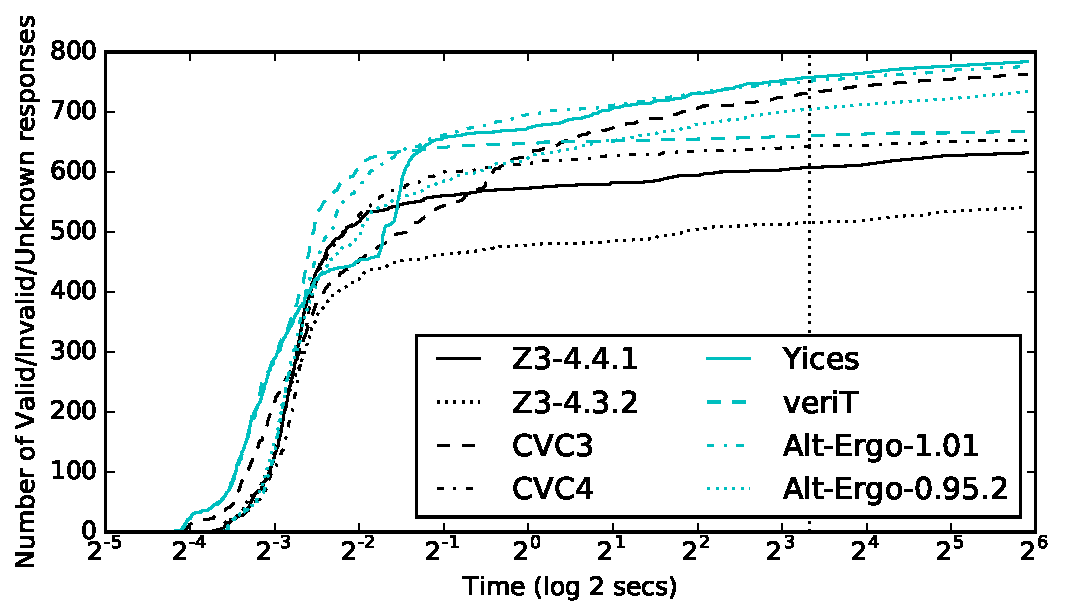
\includegraphics[width=\linewidth]{line_graph}
	\caption{The cumulative number of \textit{Valid/Invalid/Unknown} responses for each solver. The plot uses a logarithmic scale on the time axis for increased clarity at the low end of the scale. The chosen timeout limit of 10 secs (\textit{dotted vertical line}) includes 99\% of each solver's useful responses}
	\label{fig:line_graph}
\end{figure}



%----------------------------------------------------------------------------------------

%perhaps include a system diagram at this point


%Container-based timings using \textit{BenchExec}







\subsection{Prover output}





